
\section{Motivation}



\begin{frame}{Deep Learning: everything is a vector}
	\vspace{-15pt}
	
  \begin{center}
  	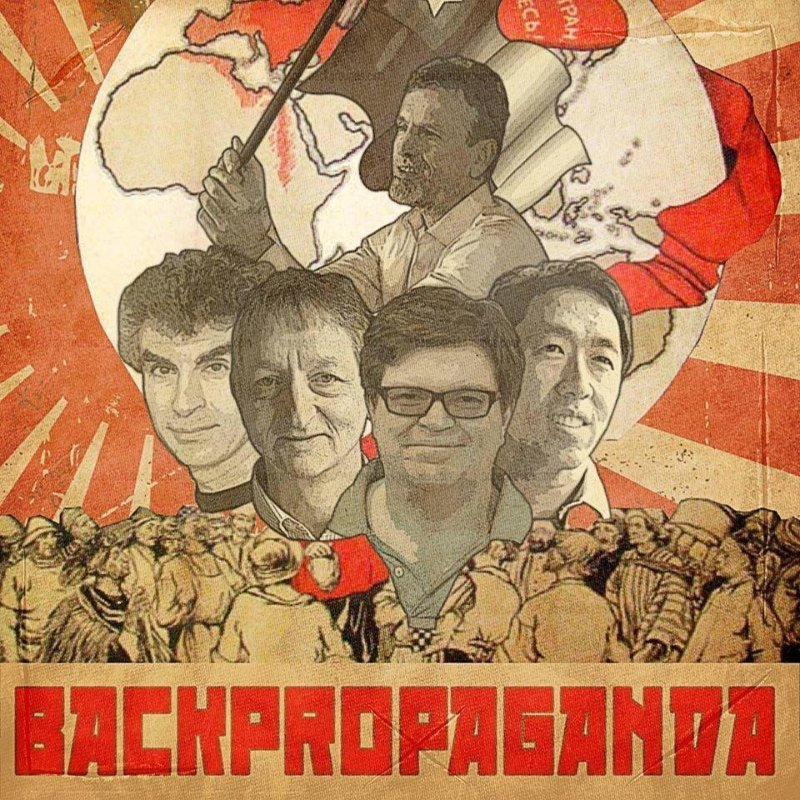
\includegraphics[width=0.59\textwidth]{figures/backprop}
  \end{center}
   
%{  \footnotesize
%  Image source: \url{https://www.linkedin.com/feed/update/urn:li:activity:6442811914803380224}
% } 

\end{frame}


\begin{frame}{Linguistic Structures and Graphs}
	
	\begin{itemize}
		\item (Written) language is a \alert{symbolic system}
	\end{itemize}
	
	
	
\end{frame}


%
\begin{frame}{Graph Matrix Duality}
	\vspace{-25pt}
	
  \begin{center}
  	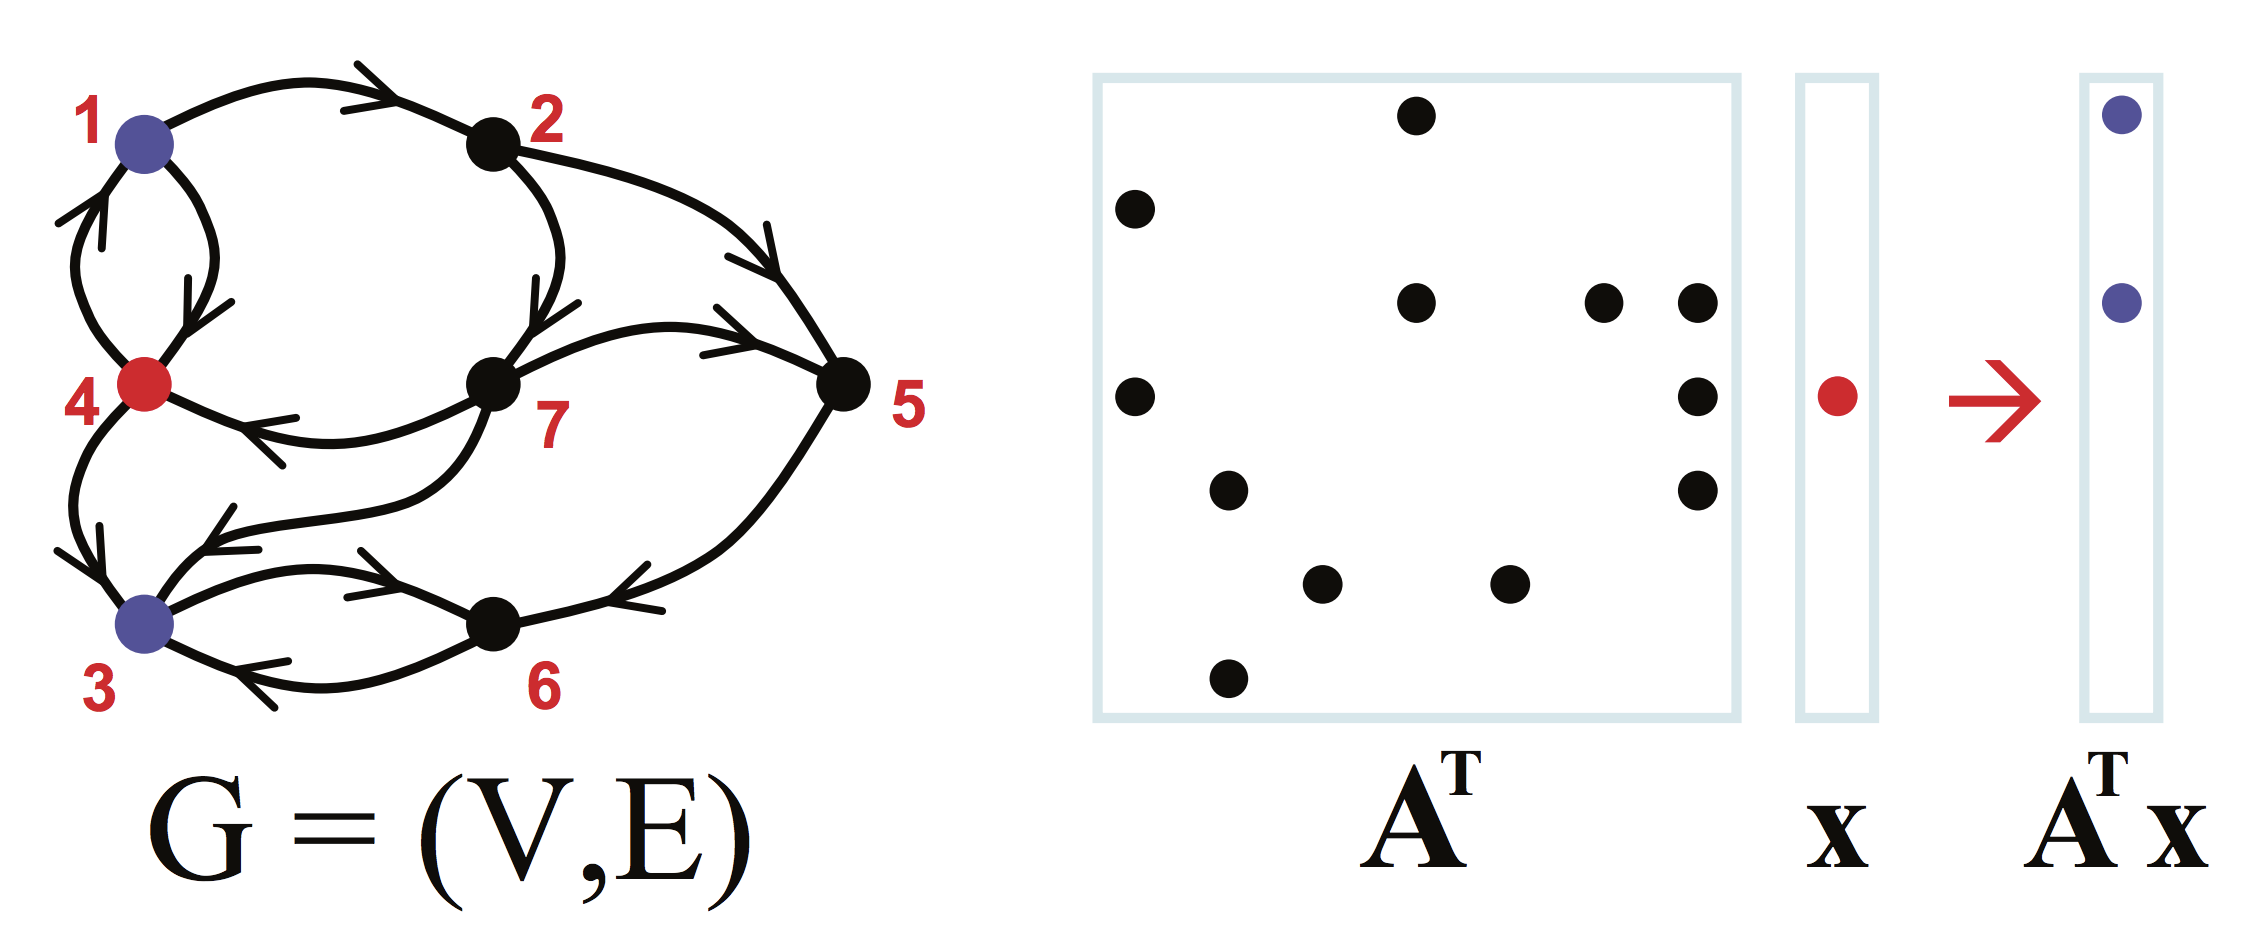
\includegraphics[width=0.99\textwidth]{figures/graph2matrix}
  \end{center}
  
  \pause 

  \begin{itemize}
  	\item   Adjacency matrix $\mathbf{A}$ is dual with the corresponding graph $G$.
  	\pause 
  	\item Vector matrix multiply $\mathbf{A}^T\mathbf{x}$ is dual with breadth-first search.
  \end{itemize}
% 
%{  \footnotesize
%  Image source: \cite{kepner2011graph}
% } 
%
\end{frame}


\begin{frame}{Goal}

  \begin{enumerate}
  	\item Learn the interpretable symbolic structures from text in an unsupervised way, which are \alert{more complex than tokens and lemmas}.
  	\pause 
  	\item Represent the learned structures in the vector form.
  	\pause 
  	\item Use the vector representations instead/in addition to word embedding the deep learning applications. 
  	\pause 
  	\item More complex structures could improve performance, but also provide better interpretability of the deep learning models. 
  	
  \end{enumerate}

\end{frame}
